\nowdb\ is a kind of database.
It merges the concepts
of \term{graph} and \term{timeseries} database.
Timeseries databases typically have simple
data models centred around timelines
consisting of pairs of the form
$(timestamp,value)$
with additional $tags$ to
distinguish thematically different timelines.
An example may be a weather forecast
application with timelines describing
temperature, humidity and air pressure
at certain locations. The values would
reflect these measurements and timestamps
would refer to the points in time when
the measurements were taken. Tags would
be used to distinguish timelines
(temperature, humidity, pressure) and
to identify the location from where the
respective measurement comes.

Timeseries databases shine in 
fast processing of large volumes of
data with similar and, typically, simple structure.
They are, typically, not good at complex
data models like relational databases.

This is where the graph model enters the scene.
Graph databases are especially good
at efficiently handling
data with growing complexity.
They are very similar to relational
databases, but replace the set-theoretic
fundament of relational databases by
graph theory. Graph databases do not deal
with relations over sets, but with
sets of vertices that are connected
by edges. In a Twitter-like application,
vertices may represent users, while
edges may be used to model
the connections between users such as
\term{following}.
Applications built on top of graph databases
typically focus on finding relations
between vertices; a goal may be to decide
whether a user $A$ belongs to the network
of a user $B$ where a follower of a
follower of $B$ is considered part of
$B$'s network. Another challenge may be
to compute how many users have seen
a certain tweet or how many users
see tweets of user $A$ in general.

Edges are formally equivalent to relations,
but more flexible. A Relational database
expresses the relation between entities
in terms of \term{foreign keys}.
That is, one entity stores a reference
to another entity in its physical
representation.
An example may be the relation
between a $product$ and its $supplier$.
A relational database would store
the \term{primary key} of the supplier
in the product.
The relation is then be built into
the product table.

A graph database would express this relation
by means of an edge between the two entities.
The entities themselves would not be touched.
There would be instead a separate entity,
\viz\ the edge table, that would link
product and supplier.

\begin{minipage}{\textwidth}
The following diagram shows the logical
relation between supplier and product and,
below on the left-hand side, its relational
interpretation and, on the right-hand side,
the graph interpretation:

\begin{center}
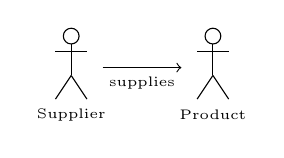
\begin{tikzpicture}
\draw (0.1,2.3) circle (0.1cm); % head
\draw (0.1,2.2) -- (0.1,1.8);   % body
\draw (-0.1,2.1) -- (0.3,2.1);  % arms
\draw (0.1,1.8) -- (-0.1,1.5);  % left leg
\draw (0.1,1.8) -- (0.3,1.5);   % right leg
\node [font=\tiny,align=center] (sup) at (0.1,1.3) {Supplier};

\draw (1.9,2.3) circle (0.1cm); % head
\draw (1.9,2.2) -- (1.9,1.8);   % body
\draw (1.7,2.1) -- (2.1,2.1);   % arms
\draw (1.9,1.8) -- (1.7,1.5);  % left leg
\draw (1.9,1.8) -- (2.1,1.5);   % right leg
\node [font=\tiny,align=center] (prod) at (1.9,1.3) {Product};

\draw [->] (0.5,1.9) -- (1.5,1.9);  % edge
\node [font=\tiny,align=center] (edg) at (1.0,1.7) {supplies};
\end{tikzpicture}

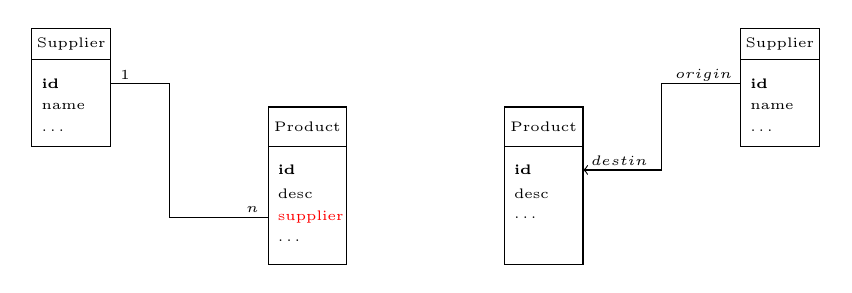
\begin{tikzpicture}
\draw (0,3) rectangle (1,1.5);
\draw (0,3) rectangle (1,2.6);
\node [font=\tiny,align=center] (sup) at (0.5,2.8) {Supplier};
\node [font=\tiny,align=center,anchor=west] (sup1) at (0,2.3) {\textbf{id}};
\node [font=\tiny,align=center,anchor=west] (sup2) at (0,2.0) {name};
\node [font=\tiny,align=center,anchor=west] (sup3) at (0,1.7) {\dots};

\draw (3,2) rectangle (4,0);
\draw (3,2) rectangle (4,1.5);
\node [font=\tiny,align=center] (prod) at (3.5,1.75) {Product};
\node [font=\tiny,align=center,anchor=west] (sup1) at (3,1.2) {\textbf{id}};
\node [font=\tiny,align=center,anchor=west] (sup2) at (3,0.9) {desc};
\node [font=\tiny,align=center,anchor=west,text=red] (sup2) at (3,0.6) {supplier};
\node [font=\tiny,align=center,anchor=west] (sup3) at (3,0.3) {\dots};

\draw (1,2.3) -- (1.75,2.3) -- (1.75,0.6) -- (3,0.6);
\node [font=\tiny,align=center,anchor=west] (one) at (1,2.4) {1};
\node [font=\tiny,align=center,anchor=west] (n) at (2.6,0.7) {$n$};

\draw (9,3) rectangle (10,1.5);
\draw (9,3) rectangle (10,2.6);
\node [font=\tiny,align=center] (sup) at (9.5,2.8) {Supplier};
\node [font=\tiny,align=center,anchor=west] (sup1) at (9,2.3) {\textbf{id}};
\node [font=\tiny,align=center,anchor=west] (sup2) at (9,2.0) {name};
\node [font=\tiny,align=center,anchor=west] (sup3) at (9,1.7) {\dots};

\draw (6,2) rectangle (7,0);
\draw (6,2) rectangle (7,1.5);
\node [font=\tiny,align=center] (prod) at (6.5,1.75) {Product};
\node [font=\tiny,align=center,anchor=west] (sup1) at (6,1.2) {\textbf{id}};
\node [font=\tiny,align=center,anchor=west] (sup2) at (6,0.9) {desc};
\node [font=\tiny,align=center,anchor=west] (sup3) at (6,0.6) {\dots};

\draw [->] (9,2.3) -- (8,2.3) -- (8,1.2) -- (7,1.2);
\node [font=\tiny,align=center,anchor=west] (origin) at (8.05,2.4) {$origin$};
\node [font=\tiny,align=center,anchor=west] (destin) at (6.98,1.32) {$destin$};
\end{tikzpicture}
\end{center}
\end{minipage}

Graph databases are therefore more flexible.
It is easily possible to add new relations
without the need to change the structure or
the data of the entities involved. Also,
there may be more than one relation holding
between two entities, for instance, at
different points in time. There is also
no difference between $1:n$ and $n:m$ relations
like in relational databases. 

In \nowdb\ edges are not only
used to express relations,
but also to add information to vertices.
This additional information
is user-defined, but always
timestamped.
Since edges are optimised
for fast processing of high data volumes,
this brings the advantages of timeseries databases
to the underlying graph model.

Indeed, \nowdb\ aims to provide the
performance advantages of timeseries databases
using concepts from graph databases
to allow more complex data models
than usually seen with timeseries databases.
\nowdb\ can thus be applied to a wider
range of applications than pure
timeseries databases without losing
their performance advantage.

\nowdb\ is in particular strong with
data that can be organised in some variant of the
\term{star} or \term{snowflake schema}. Relations between
fact tables and dimensional tables
are expressed in terms of
timestamped edges
between dimensional vertices of
arbitrary complexity that, themselves, 
can be related to each other by
simple, unstamped edges.

In contrast to traditional
\term{star schema} applications,
\nowdb\ is not limited to data analysis.
Many features stress real-time data
processing providing \term{publish and subscribe},
online data filtering and integration with big-data
infrastructure.

This manual documents the main features
of the database and discusses important
use cases. The next chapter provides
a \term{Quick Start} tutorial that helps
understanding the concepts behind \nowdb\
and introduces the most important tools.
The chapter will close
with an overview of the remaining
chapters of this document.

\comment{
Throughout the document, the reader will encounter
red comments like this one.
These comments aim to clarify the current state
of the prototype. They, in particular, draw
attention to features that are not yet available
or to shortcomings of their current implementation.
}

